\section{L2 Normalization} \label{sec:L2_Normalization}

\begin{figure}[!hbt]
    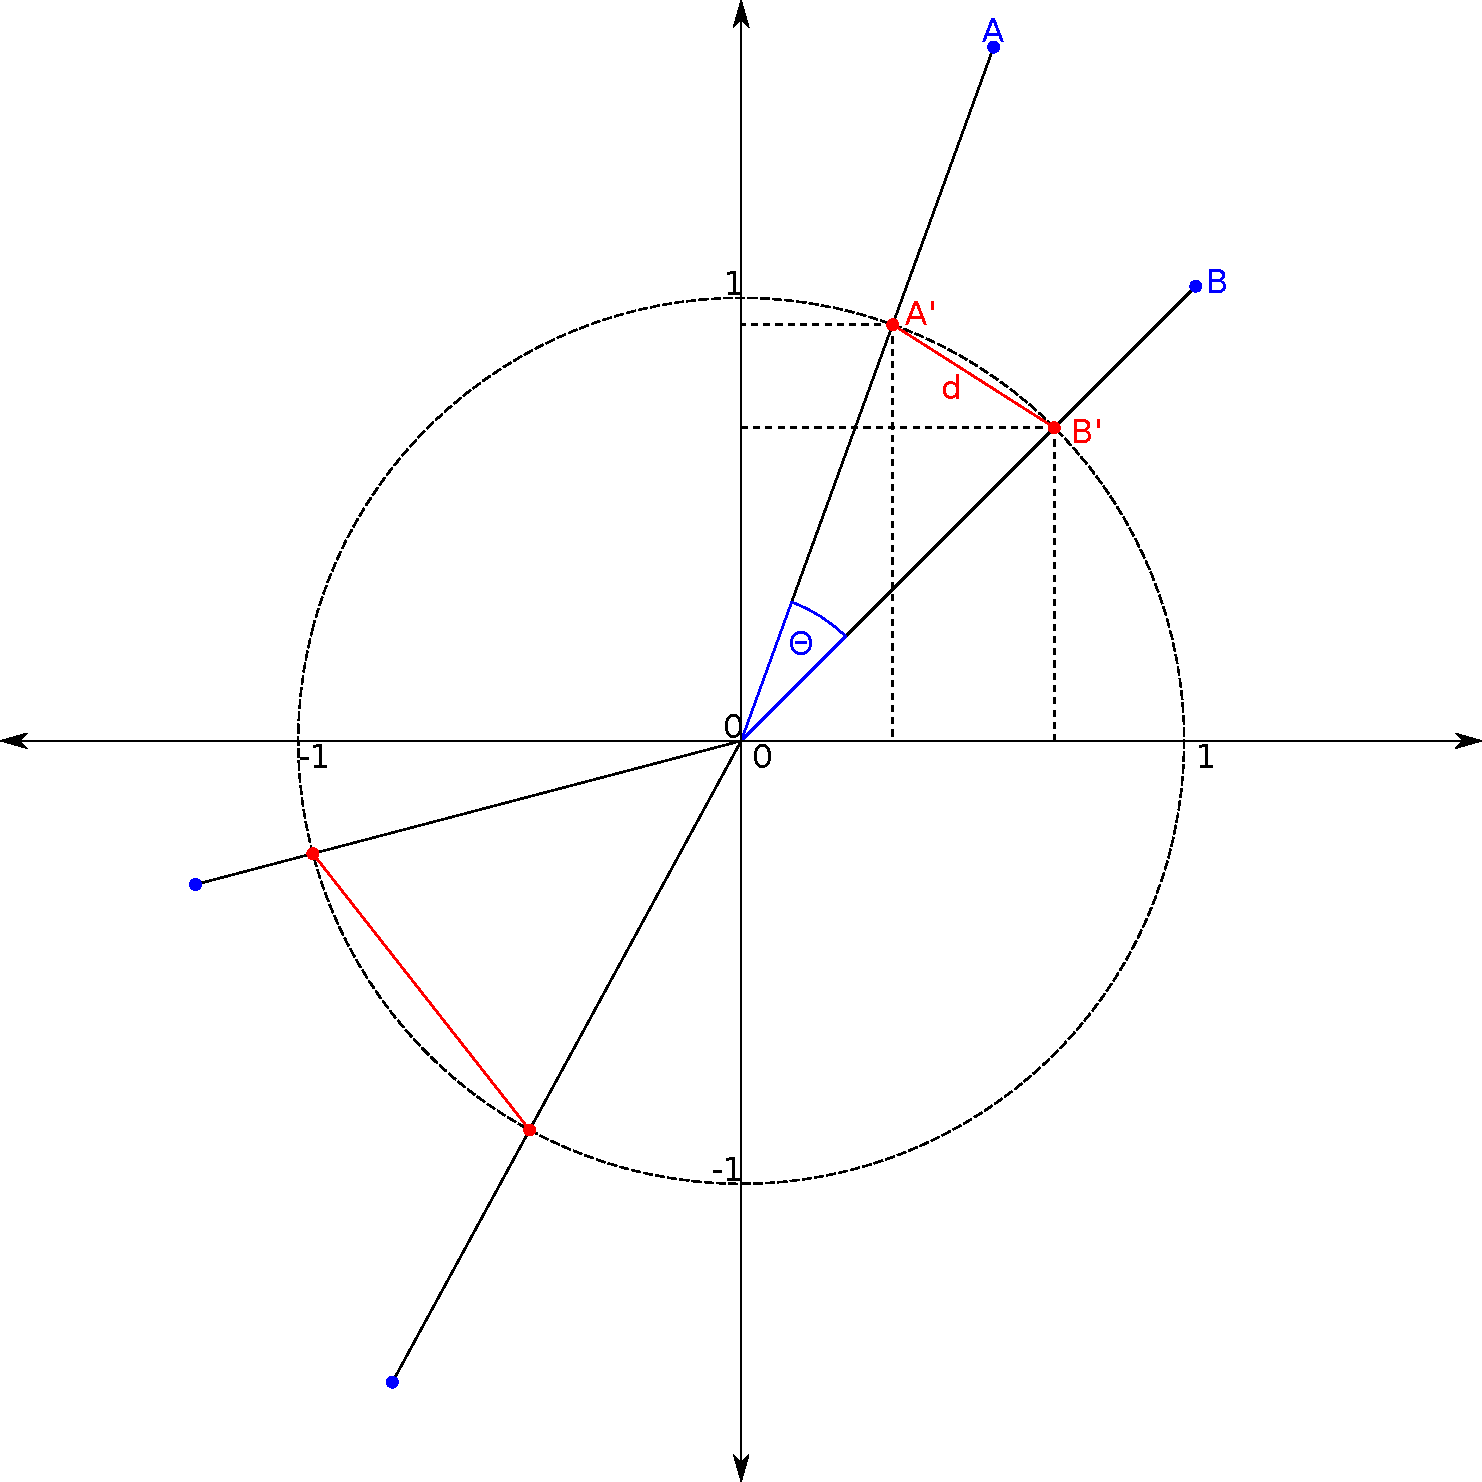
\includegraphics[width=\dimexpr\textwidth-2\fboxsep-2\fboxrule,fbox]{Extra_Graphics/L2_Euclidean.pdf}
    \caption[Mathematical Background of L2 Normalisation]{\textbf{Mathematical Background of L2 Normalisation.} .}
    \label{fig:L2_Normalisation_Background}
\end{figure}

\blindtext

\begin{figure}
    \begin{adjustbox}{minipage=\dimexpr\textwidth-2\fboxsep-2\fboxrule,fbox}
        \begin{subfigure}[b]{0.475\textwidth}
            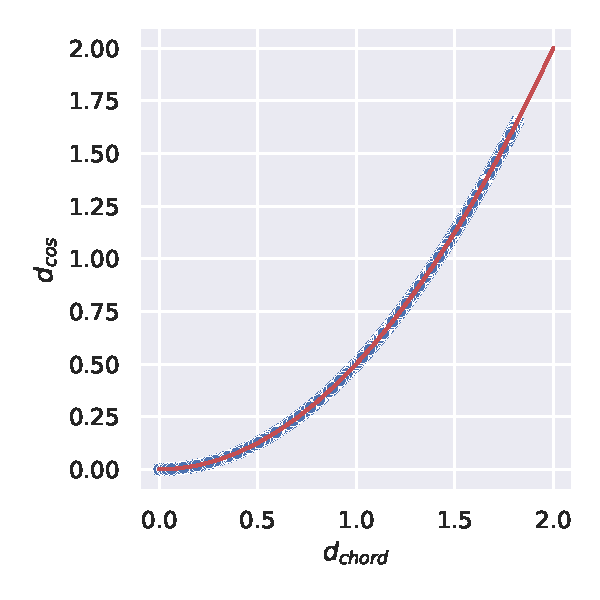
\includegraphics[width=\textwidth]{PCA/Difference_Distance_Calculation.pdf}
            \caption[Dimension Reduction with \Acrshort{PCA}]{\textbf{Dimension Reduction with \Acrshort{PCA}}}
            \label{subfig:Normalisation_PCA}
        \end{subfigure}
        \hfill
        \begin{subfigure}[b]{0.475\textwidth}
            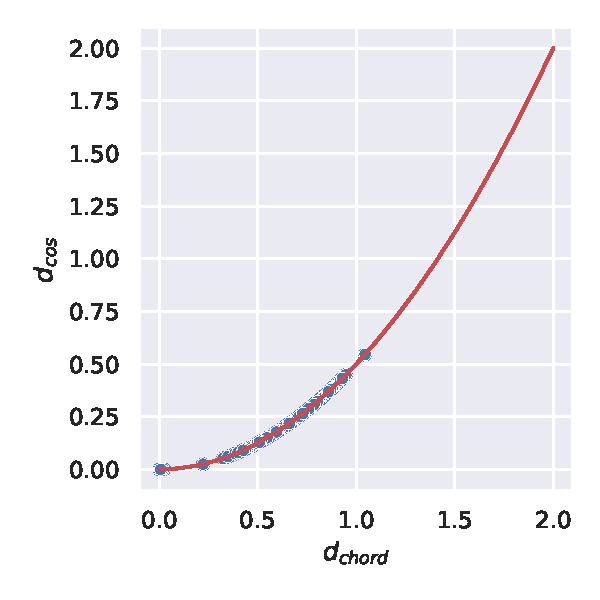
\includegraphics[width=\textwidth]{UMAP/Difference_Distance_Calculation.pdf}
            \caption[Dimension Reduction with \Acrshort{UMAP}]{\textbf{Dimension Reduction with \Acrshort{UMAP}}}
            \label{subfig:Normalisation_UMAP}
        \end{subfigure}
    \end{adjustbox}
    \caption[Cosine Distance Approximation with L2 Normalisation]{\textbf{Cosine Distance Approximation with L2 Normalisation.} .}
    \label{fig:Normalisation_Methods}
\end{figure}

\blindtext